% !TEX root=ManualTFG.tex

\chapter{Marco Teórico}\label{MarcoTeórico}
Para comprender en profundidad el desarrollo de este proyecto y justificar las decisiones adoptadas durante su diseño e implementación, resulta imprescindible establecer 
una base teórica que aborde los conceptos y tecnologías implicadas. Este marco teórico tiene como finalidad proporcionar una visión general sobre las 
infraestructuras de red en entornos hospitalarios, protocolos de comunicación, seguridad y tecnologías específicas para entornos sanitarios.

\section{Arquitectura de Redes Hospitalarias}
El correcto diseño de una infraestructura de red en entornos hospitalarios resulta esencial para garantizar la continuidad de los servicios asistenciales, la 
integridad de los datos clínicos y la seguridad de los dispositivos conectados. La particularidad de estas redes radica en la coexistencia de distintos tipos de 
tráfico (administrativo, clínico, de invitados y de dispositivos médicos), lo que exige una arquitectura flexible, segmentada y altamente disponible.

\subsection{Segmentación de la Red}
La segmentación mediante VLANs permite aislar el tráfico de diferentes áreas o servicios, mejorando la seguridad y el rendimiento. 
Cada VLAN constituye un dominio de difusión (broadcast) independiente, permitiendo la aplicación de políticas específicas y reduciendo la propagación de tráfico innecesario.

\subsection{Modelo Jerárquico de Red}
Las redes hospitalarias adoptan un modelo jerárquico de tres capas que optimiza el rendimiento, escalabilidad y mantenimiento. Esta arquitectura (Figura \ref{fig:3capas}) se compone de:
\begin{itemize}
    \item \textbf{Capa de Núcleo (Core):} Proporciona conectividad de alta velocidad entre diferentes áreas internas del hospital y acceso a servicios externos. Se encarga de 
    interconectar los switches de distribución con los routers principales y gestionar el tráfico entre las distintas subredes.
    \item \textbf{Capa de Distribución:} Actúa como intermediaria entre la capa de acceso y la capa de núcleo, gestionando el tráfico local y balanceando la carga
    entre los distintos switches de núcleo. También implementa políticas de seguridad, segmentación de tráfico y control de acceso, permitiendo la comunicación entre las distintas 
    VLANs y subredes del hospital.
    \item \textbf{Capa de Acceso:} Conecta los dispositivos finales, como estaciones de trabajo, impresoras y dispositivos médicos. Esta capa se encarga de proporcionar
    conectividad a los usuarios y dispositivos, permitiendo el acceso a los recursos de red y servicios compartidos. 
\end{itemize}
Esta estructura optimiza el rendimiento, la escalabilidad y la facilidad de mantenimiento, aspectos críticos en entornos hospitalarios donde la disponibilidad y la seguridad son prioritarias.
\begin{figure}[H]
    \centering
    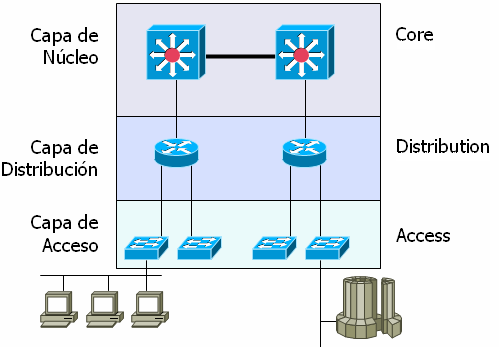
\includegraphics[width=0.5\textwidth]{Imágenes/modelo a tres capas.png}
    \caption{Modelo Jerárquico de Tres Capas}
    \label{fig:3capas}
\end{figure}

\section{Protocolos de Enrutamiento Dinámico}
En redes hospitalarias con múltiples sedes interconectadas y una estructura de red segmentada y redundante, resulta imprescindible contar con mecanismos que permitan 
gestionar automáticamente las rutas entre dispositivos y subredes. Los protocolos de enrutamiento dinámico son esenciales para garantizar la conectividad, optimizar el 
tráfico de red y asegurar una rápida convergencia ante cambios en la topología.

\subsection{Open Shortest Path First (OSPF)}
\label{subsec:ospf}
OSPF es un protocolo de enrutamiento de estado de enlace ampliamente utilizado en redes hospitalarias por su capacidad de rápida convergencia y soporte para redes complejas. 
Utiliza el algoritmo de Dijkstra para calcular rutas óptimas y mantiene una base de datos topológica completa en cada router, lo que permite una gestión eficiente y escalable 
del enrutamiento interno \cite{cisco-ospf}.
\\ \\
\textbf{Funcionamiento Básico:}
\begin{itemize}
    \item Cada router mantiene una \ac{LSDB} con información topológica completa de la red.
    \item Utiliza \ac{LSA}s para intercambiar información entre routers.
    \item Calcula rutas óptimas mediante el algoritmo \ac{SPF} de Dijkstra.
\end{itemize}

\subsubsection{Algoritmo de Dijkstra}
El algoritmo de Dijkstra, implementado en OSPF, calcula la ruta más corta entre nodos considerando los costos de enlace, lo que resulta esencial para garantizar la disponibilidad 
y eficiencia en la transmisión de datos críticos en hospitales.

\section{Protocolos de Redundancia y Alta Disponibilidad}
En entornos críticos como el hospitalario, donde la disponibilidad continua de la red es indispensable para garantizar la atención sanitaria y el acceso a información 
clínica, resulta fundamental implementar mecanismos que eviten la pérdida de servicio ante posibles incidencias en enlaces o dispositivos de red.
\\ \\
Para ello, se utilizan protocolos de redundancia y alta disponibilidad, que permiten asegurar la continuidad de la conectividad y minimizar los tiempos de caída mediante 
la conmutación automática ante fallos.

\subsection{Hot Standby Router Protocol (HSRP)}
\label{subsec:hsrp}
HSRP es un protocolo propietario de Cisco que proporciona redundancia de gateway mediante la creación de un router virtual. Un router activo gestiona el tráfico, mientras que uno 
o más routers en standby asumen el control en caso de fallo, asegurando la continuidad del servicio \cite{cisco-hsrp}. \\ \\

\textbf{Arquitectura HSRP:}
\begin{itemize}
    \item \textbf{Router Activo:} Un router se designa como activo y gestiona el tráfico hacia el gateway virtual.
    \item \textbf{Router Pasivo (Standby):} Otro router se configura como pasivo, listo para asumir el rol de activo en caso de fallo del router activo.
    \item \textbf{Router Pasivo (Listen):} El tercer router se configura como pasivo en modo listen, listo para asumir el rol de router pasivo en modo Standby en caso de fallo del router activo.
    \item \textbf{Gateway Virtual:} Se asigna una dirección IP virtual que actúa como puerta de enlace para los dispositivos de la red.
\end{itemize}
\textbf{Mecanismos de Detección de Fallos:}
\begin{itemize}
    \item Paquetes Hello enviados cada 10 segundos a la dirección multicast 224.0.0.2 para detectar la disponibilidad del router activo.
    \item Dead interval para detectar routers no funcionales, que se establece en 30 segundos.
    \item Configuración de prioridades para determinar el router activo, donde el router con mayor prioridad se convierte en activo.
\end{itemize}

\subsection{EtherChannel y Agregación de Enlaces}
\label{subsec:etherchannel}
EtherChannel permite agrupar múltiples enlaces físicos en un único enlace lógico, incrementando el ancho de banda, proporcionando redundancia y balanceando la carga de tráfico. Cisco soporta tanto
 \ac{PAgP} como \ac{LACP} (estándar IEEE) para la negociación de enlaces agregados \cite{networklessons-etherchannel}. Algunos beneficios que ofrece son:

\begin{itemize}
    \item \textbf{Mayor ancho de banda:} Combina el ancho de banda de varios enlaces físicos, mejorando la capacidad de la red.
    \item \textbf{Redundancia:} Si un enlace falla, el tráfico se redistribuye automáticamente entre los enlaces restantes, garantizando la continuidad del servicio.
    \item \textbf{Balanceo de carga:} Distribuye el tráfico entre los enlaces agregados, optimizando el uso de recursos y evitando cuellos de botella.
\end{itemize}

\section{Servicios de Red Fundamentales}
Para el correcto funcionamiento de cualquier infraestructura de red, y especialmente en entornos hospitalarios donde conviven múltiples dispositivos, servicios y usuarios, 
resulta imprescindible disponer de una serie de servicios de red esenciales que garanticen la conectividad, la gestión eficiente de direcciones IP y el acceso controlado a recursos externos.

\subsection{Dynamic Host Configuration Protocol (DHCP)}
\label{subsec:dhcp}
DHCP automatiza la asignación de direcciones IP y otros parámetros de red, simplificando la gestión y reduciendo errores de configuración. En entornos hospitalarios, esto facilita la 
incorporación y administración de numerosos dispositivos médicos y administrativos. Su funcionamiento es el siguiente:
\begin{enumerate}
    \item \textbf{Descubrimiento:} El cliente envía un mensaje DHCP Discover para localizar servidores DHCP disponibles.
    \item \textbf{Oferta:} Los servidores DHCP responden con un mensaje DHCP Offer que incluye una dirección IP y otros parámetros de configuración.
    \item \textbf{Solicitud:} El cliente selecciona una oferta y envía un mensaje DHCP Request al servidor elegido.
    \item \textbf{Confirmación:} El servidor responde con un mensaje DHCP Acknowledgment, confirmando la asignación de la dirección IP.
    \item \textbf{Renovación:} Antes de que expire el tiempo de concesión, el cliente solicita una renovación de la dirección IP para continuar utilizándola.
    \item \textbf{Liberación:} Cuando el cliente ya no necesita la dirección IP, envía un mensaje DHCP Release al servidor para liberar la dirección.
\end{enumerate}

\subsection{Network Address Translation (NAT)}
\label{subsec:nat}
NAT permite que múltiples dispositivos compartan una única dirección IP pública, siendo esencial para la conectividad a Internet en redes hospitalarias \cite{cisco-hospital-design}. Los tipos principales son:
\begin{itemize}
    \item \textbf{NAT Estático:} Asocia una dirección IP privada a una dirección IP pública específica, permitiendo el acceso externo a un dispositivo concreto.
    \item \textbf{NAT Dinámico:} Asigna direcciones IP públicas de un grupo a dispositivos privados según sea necesario, optimizando el uso de direcciones IP.
    \item \textbf{\ac{PAT}:} Permite que múltiples dispositivos compartan una única dirección IP pública utilizando diferentes números de puerto para distinguir las conexiones.
\end{itemize}

\textbf{Ventajas de NAT:}
\begin{itemize}
    \item \textbf{Conservación de direcciones IP:} Permite que múltiples dispositivos utilicen una única dirección IP pública, lo que es crucial en entornos con recursos limitados.
    \item \textbf{Seguridad:} Oculta las direcciones IP internas de la red, dificultando el acceso no autorizado desde el exterior.
    \item \textbf{Flexibilidad:} Facilita la conexión a Internet de dispositivos que no requieren acceso directo desde el exterior, como impresoras o dispositivos IoMT.
\end{itemize}

\section{Seguridad de Red y Control de Acceso}
La seguridad en redes hospitalarias se ha convertido en un aspecto esencial dentro de la gestión tecnológica sanitaria, dado que en estos entornos no solo se maneja información 
crítica de carácter personal y médico, sino que además se conectan dispositivos clínicos cuyo correcto funcionamiento puede incidir directamente en la seguridad y salud de 
los pacientes. La evolución hacia infraestructuras digitales más complejas y la incorporación masiva de dispositivos médicos conectados (IoMT) ha incrementado notablemente 
la superficie de exposición a posibles ciberataques, lo que obliga a diseñar políticas de seguridad específicas, adaptadas a las necesidades de este tipo de entornos.
\\ \\
Para garantizar la seguridad de la infraestructura de red hospitalaria, se pueden usar mecanismos de control de tráfico como las Listas de Control de Acceso (ACLs) o las zonas desmilitarizadas. 

\subsection{Listas de Control de Acceso (ACLs)}
\label{subsec:acl}
Las ACLs permiten filtrar el tráfico de red según criterios específicos, como direcciones IP, protocolos o puertos. Las ACLs se configuran en los dispositivos de red (switches de capa 3 y routers) \cite{cisco-hospital-design}. Estas se 
clasifican en dos tipos principales:

\begin{itemize}
    \item \textbf{ACLs estándar:} Filtran el tráfico únicamente por dirección IP de origen, permitiendo o denegando el acceso a toda la red o a subredes específicas.
    \item \textbf{ACLs extendidas:} Permiten un filtrado más granular, considerando tanto la dirección IP de origen como la de destino, protocolos y puertos específicos.
\end{itemize}

Los componentes de una ACL incluyen:
\begin{itemize}
    \item \textbf{Sujeto:} Entidad que solicita acceso a un recurso, como un usuario o dispositivo.
    \item \textbf{Acción:} Permite o deniega el acceso al recurso solicitado.
    \item \textbf{Objeto:} Recurso al que se solicita acceso, como un servidor, base de datos o dispositivo de red.
    \item \textbf{Condición:} Criterios que determinan si se permite o deniega el acceso, como direcciones IP, protocolos o puertos.
\end{itemize}

\subsection{Secure Shell (SSH)}
\label{subsec:ssh}
SSH es un protocolo de red que permite la administración segura de dispositivos a través de una conexión cifrada \cite{cisco-hospital-design}. Sus características principales son:
\begin{itemize}
    \item \textbf{Cifrado de datos:} Protege la confidencialidad e integridad de la información transmitida, evitando que sea interceptada por terceros.
    \item \textbf{Autenticación segura:} Utiliza claves públicas y privadas para autenticar a los usuarios, garantizando que solo personal autorizado pueda acceder a los dispositivos.
    \item \textbf{Túneles seguros:} Permite crear túneles cifrados para transmitir datos sensibles, como credenciales o información médica, entre dispositivos.
\end{itemize}
\textbf{Beneficios de SSH:}
\begin{itemize}
    \item \textbf{Seguridad en la administración remota:} Facilita la gestión de dispositivos de red sin comprometer la seguridad de la información.
    \item \textbf{Protección contra ataques:} Reduce el riesgo de ataques de intermediarios (\ac{MITM}) y suplantación de identidad, asegurando que las comunicaciones sean auténticas.
    \item \textbf{Auditoría y seguimiento:} Permite registrar las actividades realizadas durante las sesiones SSH, facilitando la auditoría y el seguimiento de acciones administrativas.
\end{itemize}

\subsection{Zonas Desmilitarizadas (DMZ)}
Las zonas desmilitarizadas (DMZ) son una técnica de seguridad que permite aislar servicios accesibles desde Internet de la red interna del hospital, proporcionando una capa adicional de protección.
En entornos hospitalarios, las DMZ se utilizan para alojar servicios como servidores web, servidores de correo electrónico o aplicaciones accesibles desde el exterior \cite{dmz}.
\\ \\
También suelen incluir elementos de filtrado de tráfico como los firewalls, pero tambíen se pueden implementar configuraciones en los routers, para que simulen las funciones de los firewalls.

\textbf{Beneficios de las DMZ:}
\begin{itemize}
    \item \textbf{Aislamiento de servicios:} Permite que los servicios accesibles desde Internet estén separados de la red interna, reduciendo el riesgo de comprometer sistemas críticos.
    \item \textbf{Control de acceso:} Facilita la implementación de políticas de seguridad más estrictas para los servicios expuestos, limitando el acceso a recursos internos.
    \item \textbf{Monitoreo y detección de intrusiones:} Las DMZ permiten una mejor supervisión del tráfico entrante y saliente, facilitando la detección de actividades sospechosas.
\end{itemize}

\subsection{DHCP Snooping}
\label{subsec:dhcpsnooping}
DHCP Snooping es una característica de seguridad que protege la red contra ataques de suplantación de servidor DHCP (DHCP Spoofing). Funciona filtrando las solicitudes DHCP y
permitiendo solo aquellas provenientes de servidores DHCP autorizados \cite{cisco_dhcp_snooping}. Sus características principales son:
\begin{itemize}
    \item \textbf{Filtrado de mensajes DHCP:} Permite que solo los mensajes DHCP provenientes de servidores autorizados sean aceptados, bloqueando solicitudes maliciosas.
    \item \textbf{Prevención de ataques:} Protege contra ataques de suplantación de servidor DHCP, donde un atacante intenta responder a solicitudes DHCP con información falsa.
    \item \textbf{Registro de asignaciones:} Mantiene un registro de las asignaciones de direcciones IP realizadas por los servidores DHCP autorizados, facilitando la auditoría y el seguimiento.
\end{itemize}

\subsection{Virtual Private Network Internet Protocol Security (VPN IPSec)}
\label{subsec:ipsec}
La \ac{VPN} Internet Protocol Security (IPSec) es una tecnología que utiliza el conjunto de protocolos IPSec para crear túneles cifrados seguros a través de redes públicas, 
como Internet. Su función principal es garantizar la confidencialidad, integridad y autenticidad de los datos transmitidos entre dos puntos, protegiendo la información 
sensible frente a accesos no autorizados y ataques de intermediarios \cite{ipsec}.

\subsubsection{IPSec}
IPSec es un conjunto de protocolos que proporciona seguridad a nivel de red mediante la autenticación y cifrado de paquetes IP. Esto permite que los datos enviados desde 
un origen sean cifrados y autenticados para que solo el destinatario legítimo pueda acceder a ellos. IPSec asegura además la integridad de los datos, evitando modificaciones 
durante la transmisión \cite{ipsec}.
\subsubsection{Modos de IPSec}
IPSec opera principalmente en dos modos:
\begin{itemize}
    \item \textbf{Modo Túnel:} Protege todo el paquete IP original, incluyendo encabezado y carga útil, encapsulándolo dentro de un nuevo paquete con un encabezado IPSec. 
    Este modo es ideal para conexiones a través de redes públicas, ya que oculta la información original y proporciona un túnel seguro entre dos redes o dispositivos. 
    Es el modo utilizado por las VPN IPSec para garantizar la privacidad y seguridad de extremo a extremo \cite{ipsec}.
    \item \textbf{Modo Transporte:} Solo cifra la carga útil del paquete IP, dejando el encabezado original sin cifrar para que los enrutadores puedan dirigir el tráfico. 
    Se utiliza en redes confiables o para comunicaciones directas entre dos dispositivos, por ejemplo, en conexiones cliente-servidor dentro de una misma organización \cite{ipsec}.
\end{itemize}
\subsubsection{Funcionamiento VPN IPSec}
Una VPN IPSec crea un túnel cifrado entre dos puntos finales (por ejemplo, dos routers o un cliente y un servidor), permitiendo que los datos viajen de forma segura a través de redes 
no confiables \cite{ipsec}. El proceso incluye:
\begin{itemize}
    \item Negociación de parámetros de seguridad mediante protocolos como ISAKMP/IKE para establecer asociaciones seguras.
    \item Establecimiento de claves criptográficas para cifrar y descifrar la información.
    \item Creación del túnel VPN que encapsula y protege el tráfico IP.
    \item Transmisión segura de datos autenticados y cifrados, con protección contra ataques de repetición y suplantación.
\end{itemize}

\section{Introducción a IoMT (Internet of Medical Things)}
Internet of Medical Things (IoMT) es una evolución natural de Internet of Things (IoT) aplicada al ámbito sanitario, que permite la interconexión de dispositivos médicos, 
sensores y sistemas de información clínica a través de redes seguras. Esta tecnología posibilita la monitorización remota de pacientes, el control en tiempo real de 
parámetros fisiológicos y la gestión eficiente de recursos hospitalarios, contribuyendo a mejorar la calidad asistencial y la toma de decisiones clínicas basadas en datos 
fiables y actualizados \cite{articulo2} \cite{articulo3}. \\ \\

En la práctica hospitalaria, la \ac{IoMT} se ha consolidado como una herramienta fundamental para optimizar los procesos sanitarios, incrementando la capacidad de respuesta ante situaciones
críticas y reduciendo la carga de trabajo del personal clínico. Gracias a la integración de sensores biomédicos, dispositivos portátiles y plataformas de gestión de datos, 
los profesionales sanitarios pueden disponer de información vital en tiempo real, lo que favorece diagnósticos más precisos y tratamientos personalizados \cite{articulo3}. \\ \\

Además, el IoMT desempeña un papel esencial en la mejora de la eficiencia operativa hospitalaria. Como se recoge en la literatura, su implementación permite localizar y gestionar
equipamiento médico, optimizar la trazabilidad de pacientes y activos, y mejorar la monitorización de entornos hospitalarios críticos, como quirófanos y unidades de cuidados intensivos.
Este ecosistema conectado se apoya en tecnologías de comunicación de baja potencia y largo alcance (\ac{LPWAN}) como Sigfox, \ac{LoRa} y \ac{NB-IoT}, que proporcionan conectividad eficiente para
dispositivos médicos que requieren bajo consumo energético y cobertura extendida dentro y fuera de los centros sanitarios \cite{articulo2}. \\ \\

Desde el punto de vista arquitectónico, las soluciones IoMT han evolucionado hacia modelos distribuidos basados en edge/fog computing, donde los datos se procesan parcialmente
en pasarelas inteligentes cercanas a los dispositivos, antes de enviarse a plataformas en la nube para su almacenamiento y análisis avanzado. Este enfoque permite reducir la 
latencia, mejorar la seguridad de los datos sensibles y aliviar la carga de tráfico hacia los servidores centrales, favoreciendo la continuidad asistencial en entornos hospitalarios
con elevada demanda de recursos \cite{articulo1} \cite{articulo3}. \\ \\

El auge del IoMT también plantea desafíos en materia de seguridad, privacidad e interoperabilidad, dado que la cantidad de información médica gestionada por estos sistemas es altamente 
sensible y está sujeta a estrictos marcos normativos \cite{articulo3}. \\ \\

En definitiva, la implantación del IoMT en entornos hospitalarios representa una oportunidad estratégica para transformar la asistencia sanitaria, dotándola de mayor flexibilidad, 
capacidad predictiva y resiliencia frente a situaciones de crisis como la vivida durante la pandemia de COVID-19, donde estas tecnologías demostraron su potencial para mejorar la 
monitorización, la toma de decisiones y la gestión de recursos clínicos en tiempo real \cite{articulo3}.
